\section{Light management}
This characteristic controls the lights, so you can change the lightness of the lights through the Gateway and you can see a table with all information about lights through the Simulator.

To change the lightness of all lights, follow the next steps:
\begin{enumerate}
\item Go to the global tab for the lights in the Gateway window.

\item To change the lightness of all lights, use the slide bar or the text box (press \emph{enter} key to confirm) or predefined values to introduce a value between 0 to 100.
\begin{center}
	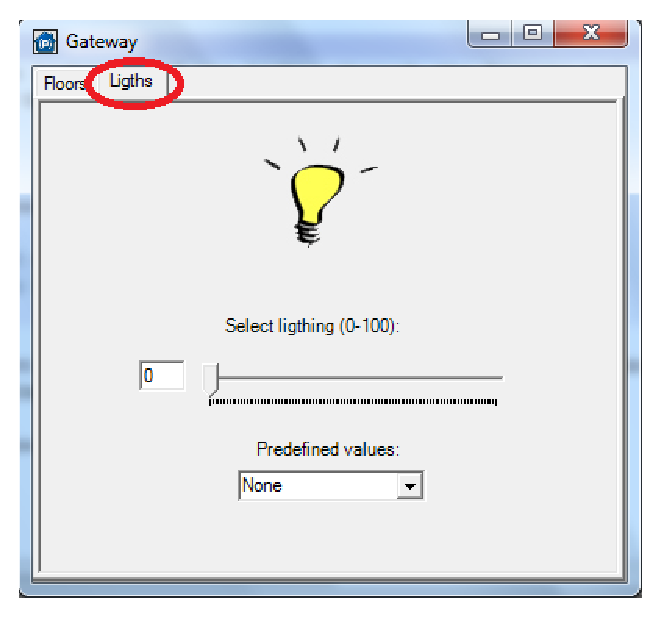
\includegraphics[width=.68\linewidth]{images/globalLight.eps}
	\\
\vspace{1cm}
\end{center}


\end{enumerate}
If you want to change the lightness of a specific light, select the room where is the light, click on the light tab and follow the same steps to modified all lights but in the current tab:
\begin{center}
	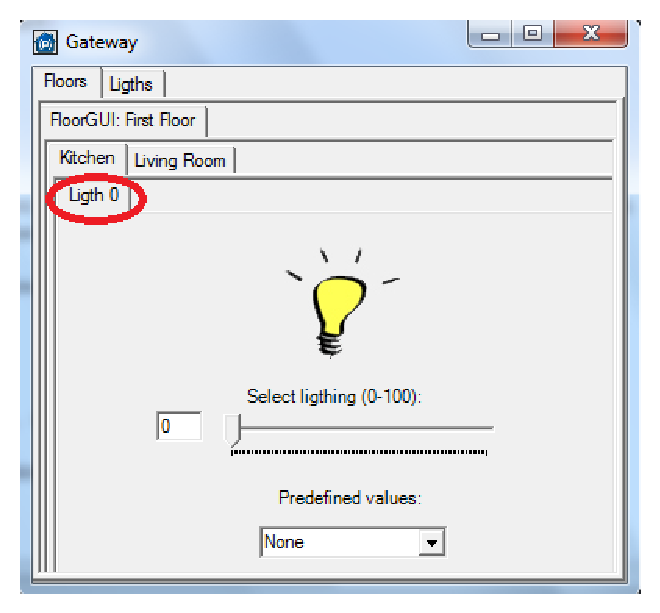
\includegraphics[width=.68\linewidth]{images/specificLight.eps}
	\\
\vspace{1cm}
\end{center}

In the Simulator window, you have a table with the identifier, room and aperture of each light:
\begin{center}
	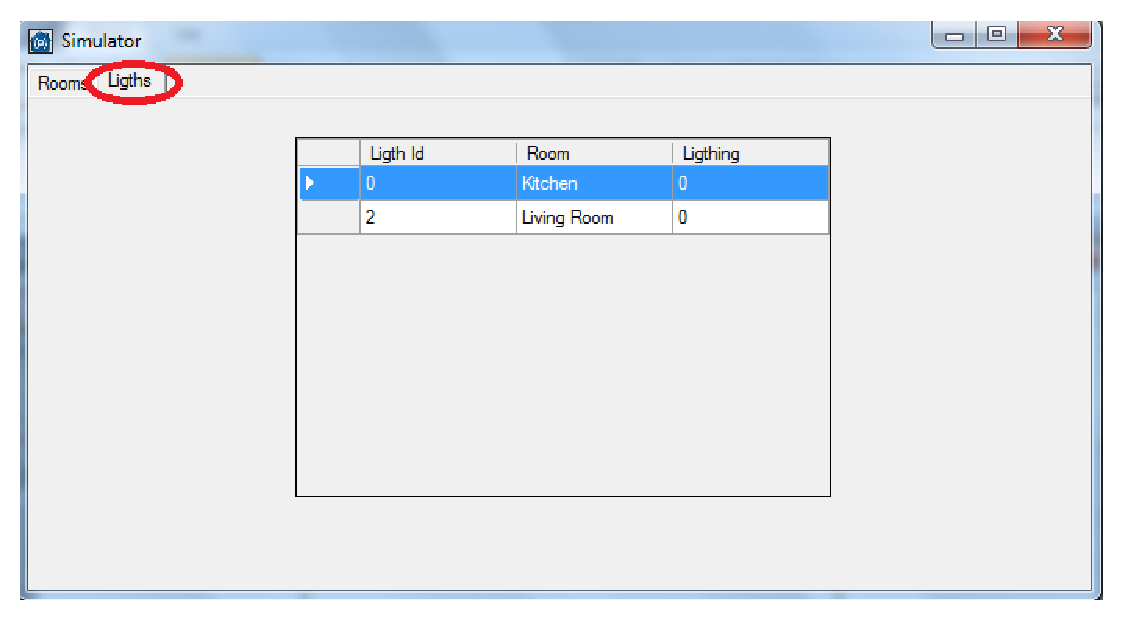
\includegraphics[width=.75\linewidth]{images/simulatorLight.eps}
	\\
\vspace{1cm}
\end{center}